\chapter{From gauging to duality in one-dimensional	quantum lattice models}\label{app:gauging}

\section{Synopsis}
It is well known that gaugings of $\mc C$-symmetric two-dimensional quantum field theories are encoded by (Frobenius) \emph{algebra objects} $A$ in $\mc C$~\cite{Fuchs2002,Bhardwaj2017}. These algebra objects specify both a gaugeable collection of topological lines and a generalised notion of \emph{discrete torsion} through their multiplication map. In this project, we extend the gauging map of Haegeman et al. ~\cite{Haegeman2014a}, initially defined for non-anomalous group symmetries, to incorporate genuine categorical symmetries and show that a choice of algebra object precisely captures the data required for this generalisation. Our construction recovers the results of ref.~\cite{Haegeman2014a} for the symmetry category $\Vect_G$, and agrees with a parallel work that discusses gauging algebra objects on the lattice, where they overlap~\cite{Seifnashri2025}. We further demonstrate that, up to constant-depth \emph{disentangling} unitary quantum circuits, the resulting gauging maps are equivalent to the duality intertwiners introduced in refs.~\cite{Lootens2021b,Lootens2022} and discussed in \cref{sec:dualities}. In addition, we consider the inclusion of symmetry-twisted boundary conditions, present several non-trivial examples, and prove the existence of a symmetric and injective matrix product state when $\mc C$ describes an anomaly-free symmetry and is thus fully gaugeable.
\newpage
\section{Reference}
\textit{From gauging to duality in one-dimensional	quantum lattice models} \par\noindent
\textbf{B. Vancraeynest-De Cuiper}, J. Garre-Rubio, F. Verstraete, K. Vervoort, D. J. Williamson, L. Lootens \par\noindent
\href{https:/doi.org/10.21468/SciPostPhys.20.4.113}{SciPost Phys. \textbf{20}, 113 (2026)}, \href{https://doi.org/10.48550/arXiv.2509.22051}{arXiv:2509.22051}
\section{Contributions of the author}
This project was conceived by José Garre-Rubio and Laurens Lootens. I derived the gauging map and the disentangling unitary transformation, in collaboration with Laurens Lootens. The gauging map in the presence of symmetry twists, as well as the examples are due to me. I wrote the manuscript, with the exception of section 5 which is written by Laurens Lootens.
%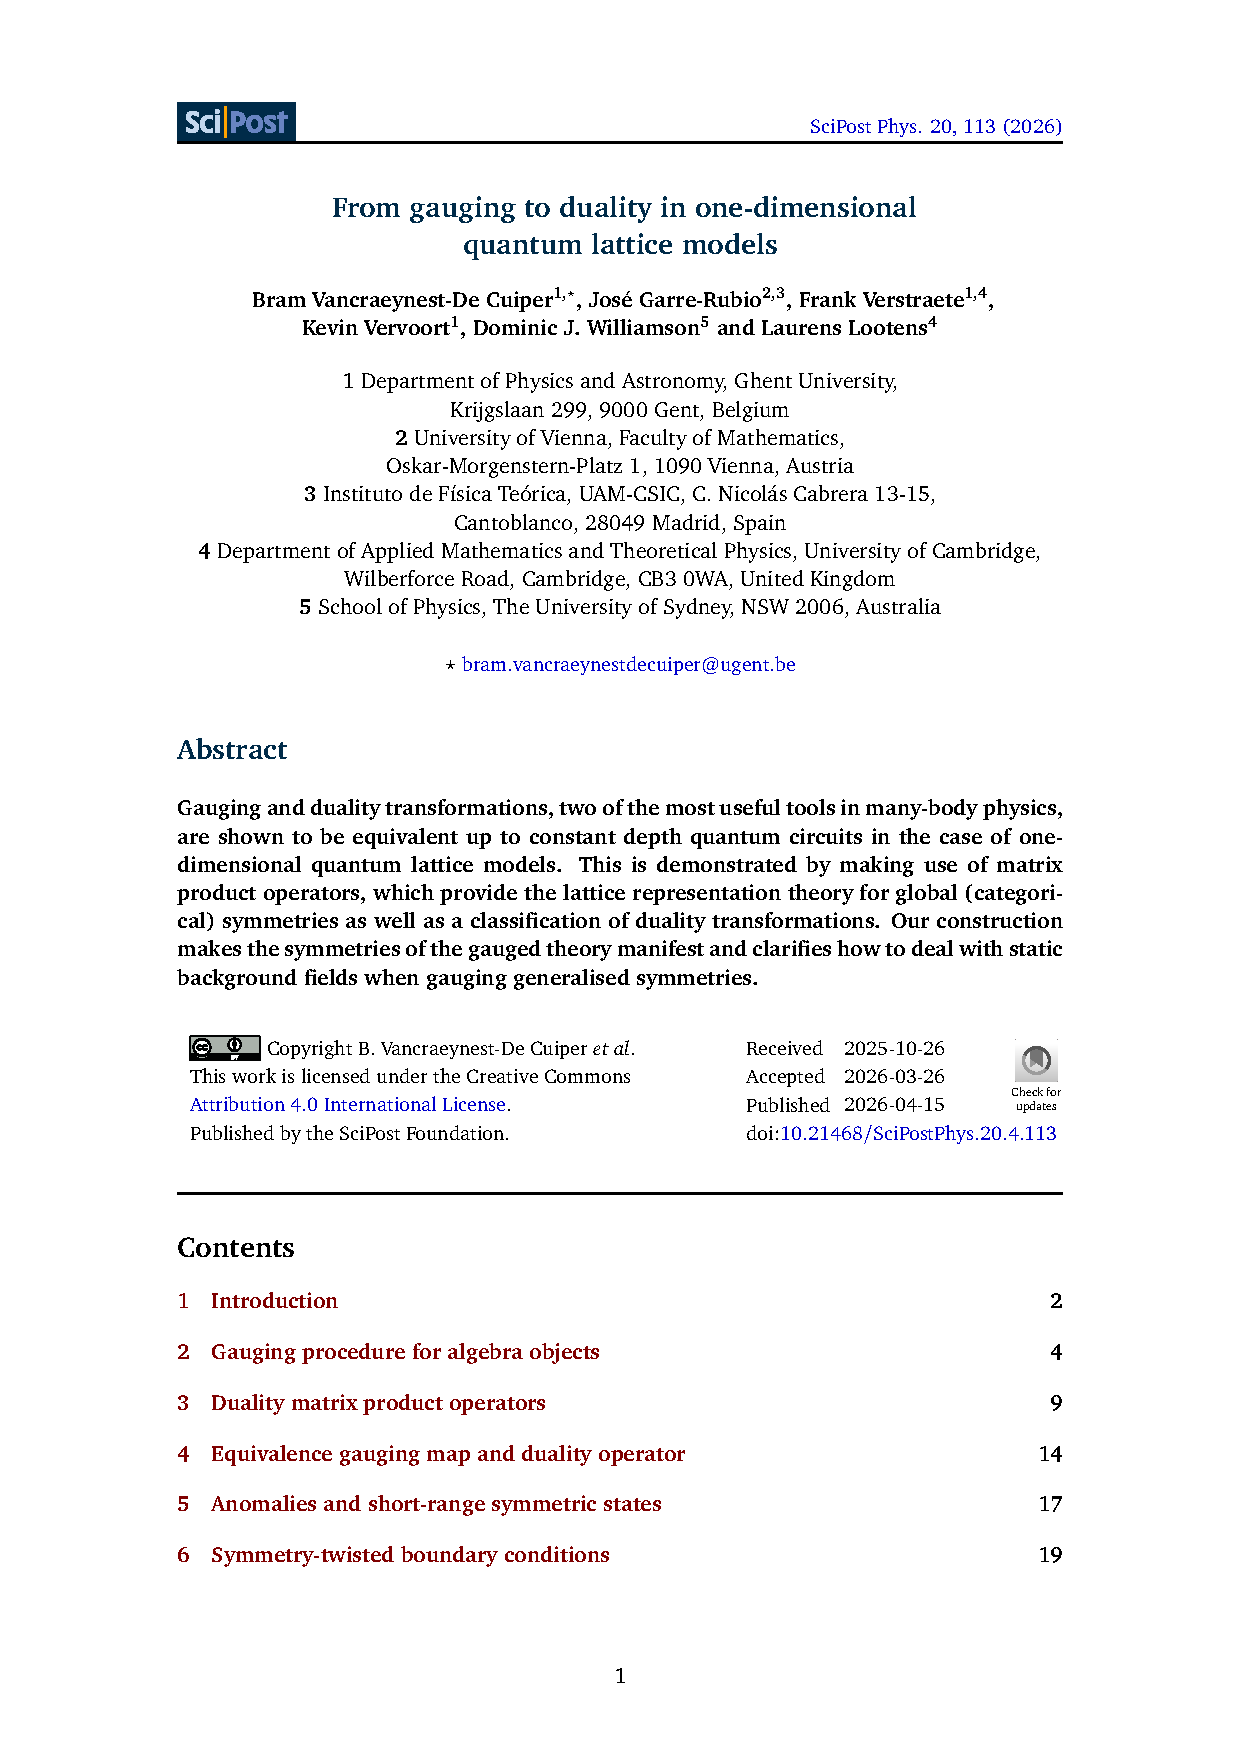
\includepdf[pages=-, trim=1.3cm 1.8cm 1.3cm 0cm, offset=-4mm 7mm, clip=true, frame=false, noautoscale=true, width=1.08\headwidth, pagecommand={}]{papers/gauging}
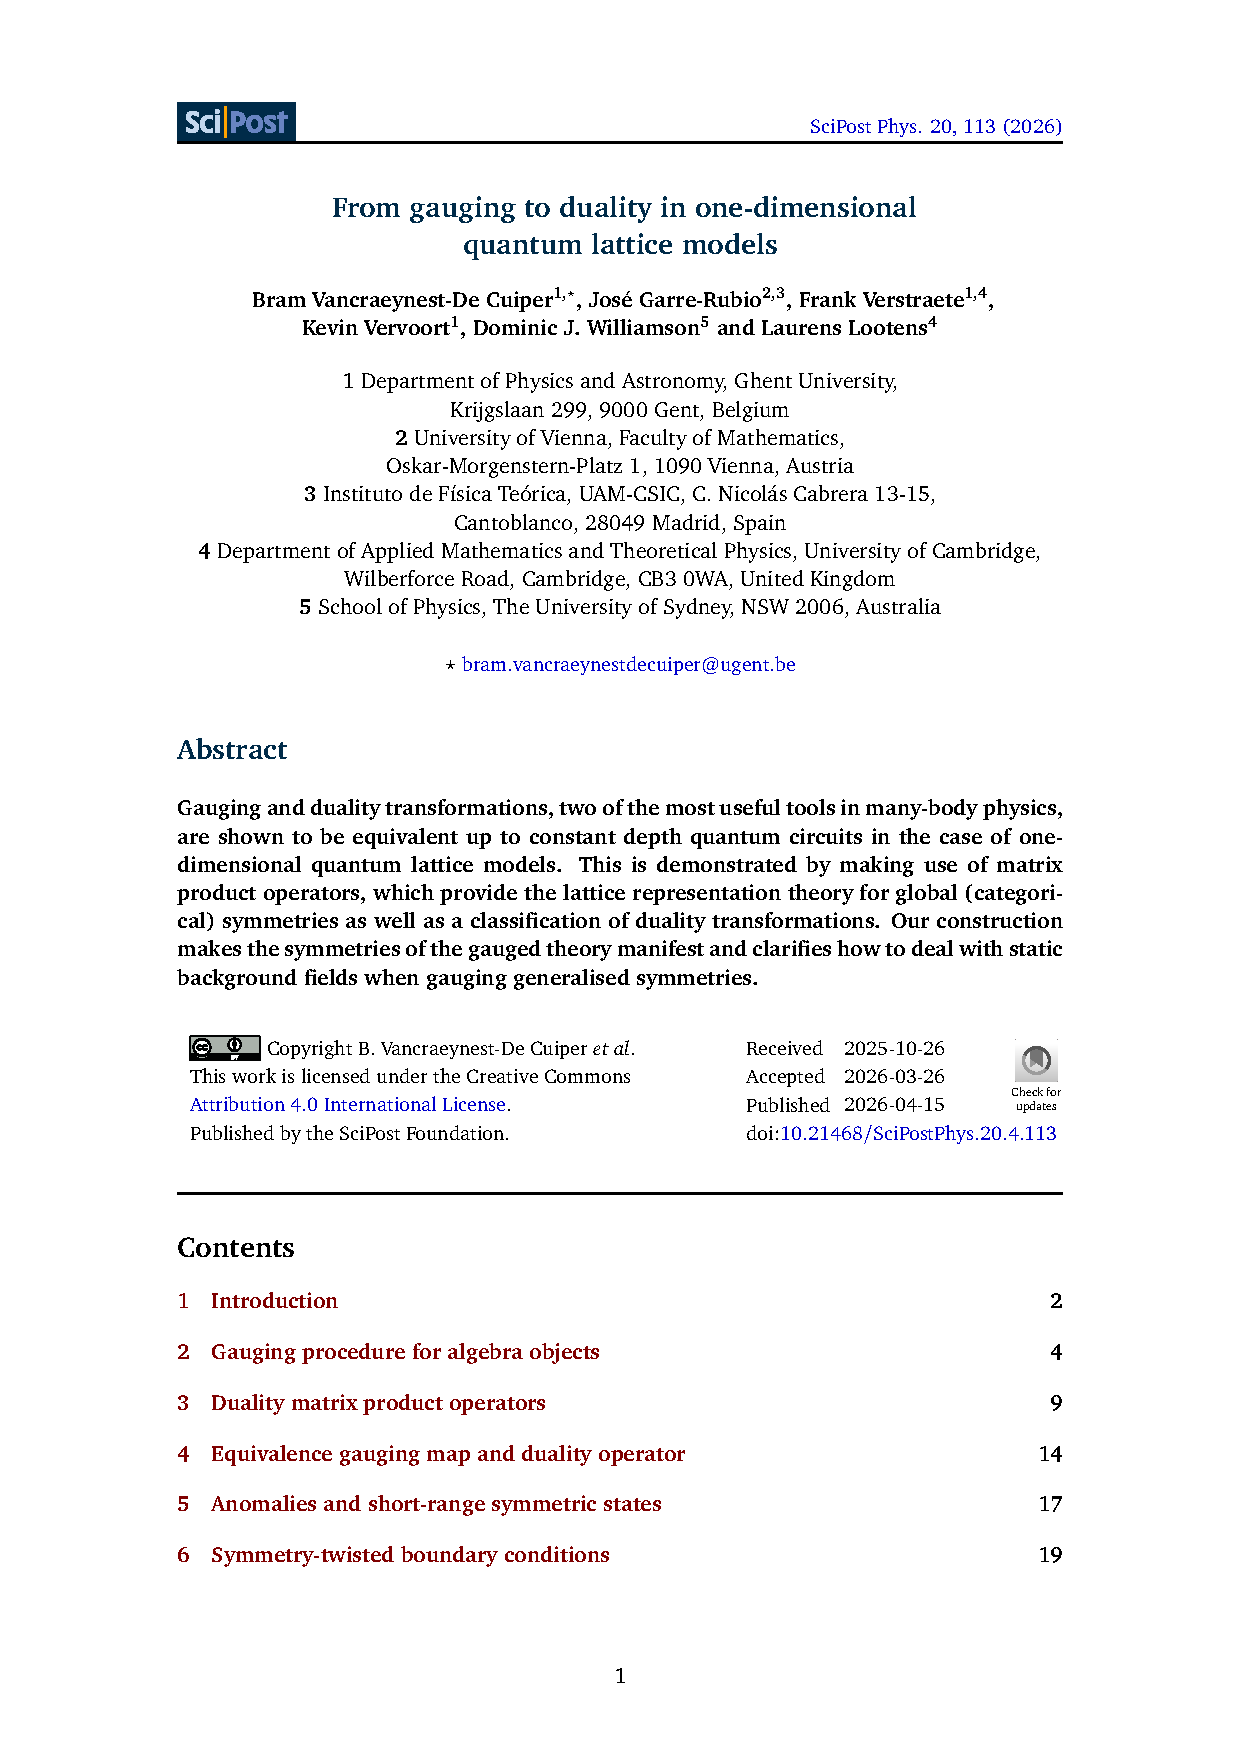
\includepdf[pages=-,
trim=25mm 20.54mm 25mm 17mm, clip=true,
noautoscale=true, height=\textheight,
offset=-0.65mm 4mm,
pagecommand={\thispagestyle{publication}}]{papers/gauging}